%
% coordsystem.tex
%
% (c) 2018 Prof Dr Andreas Müller, Hochschule Rapperswil
%
\documentclass[tikz]{standalone}
\usepackage{times}
\usepackage{amsmath}
\usepackage{txfonts}
\usepackage[utf8]{inputenc}
\usepackage{graphics}
\usetikzlibrary{arrows,intersections,math}
\usepackage{ifthen}
\begin{document}

\newboolean{showgrid}
\setboolean{showgrid}{false}

\begin{tikzpicture}[>=latex,thick]

% Povray Bild
\node at (0,0) {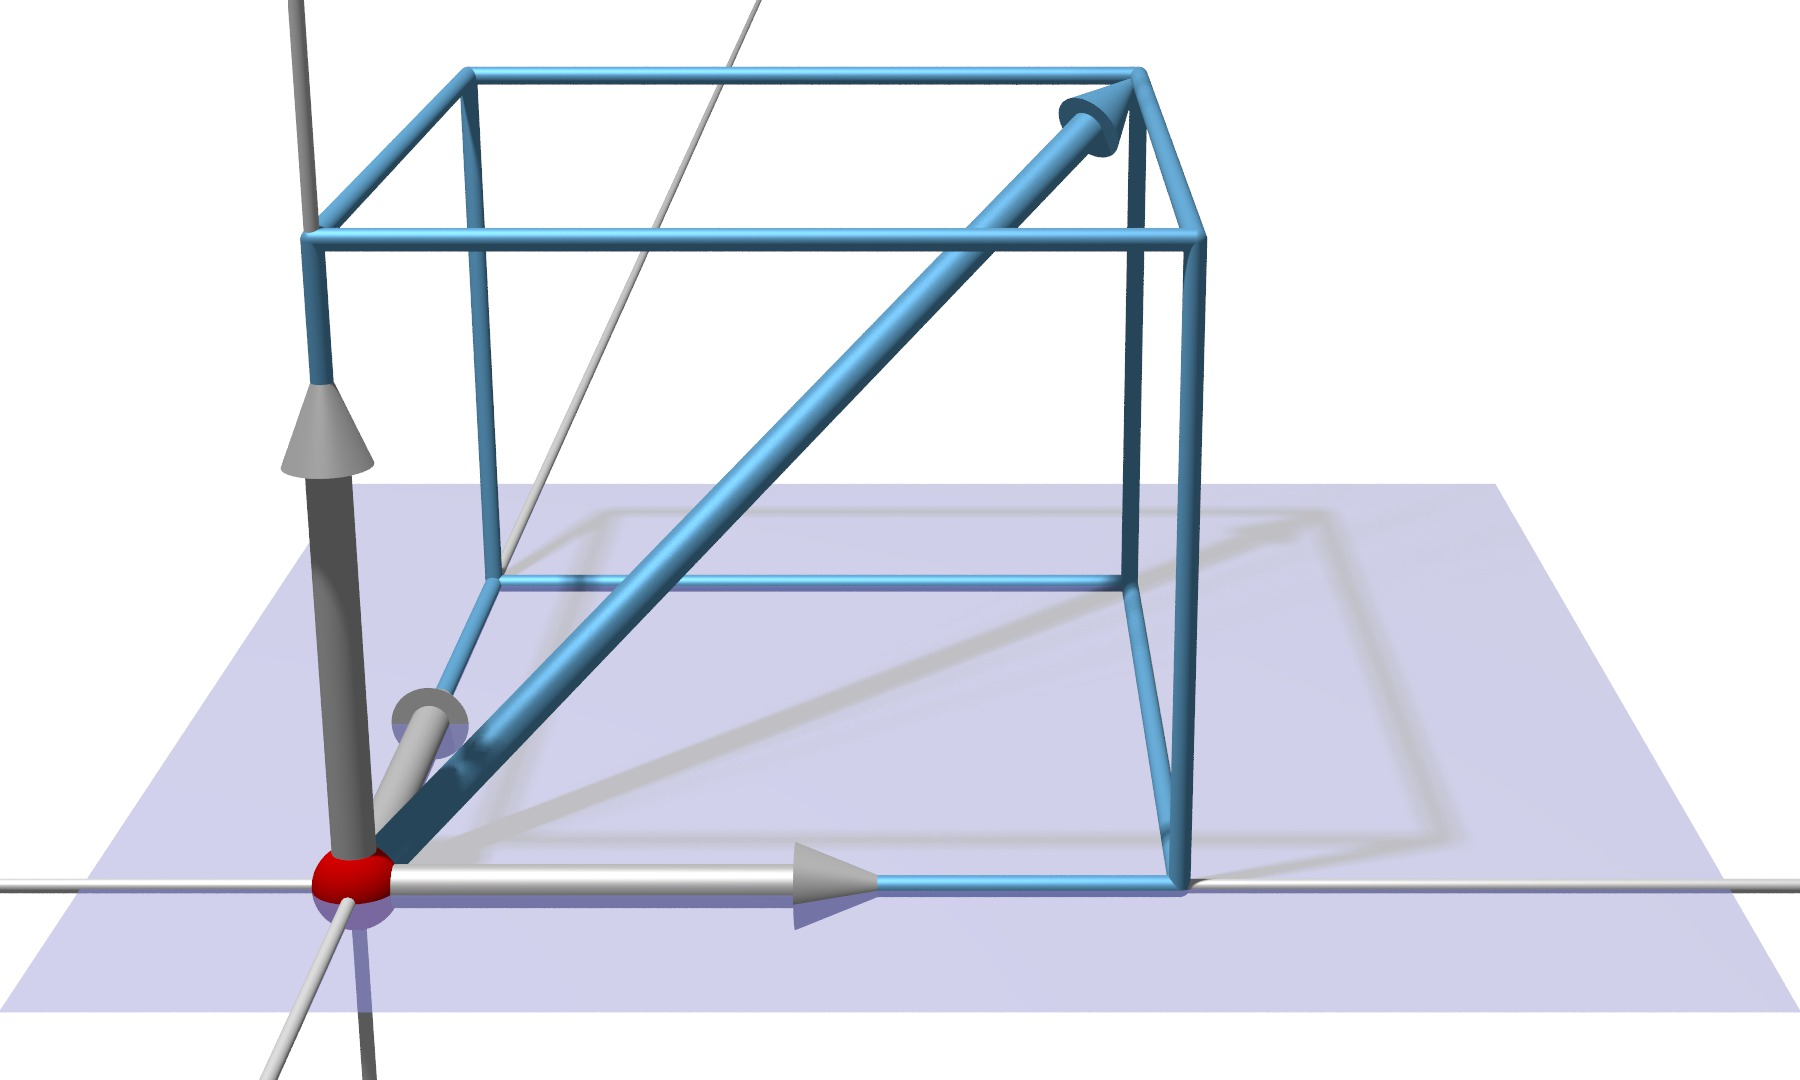
\includegraphics[width=10cm]{coordsystem.jpg}};

% Gitter
\ifthenelse{\boolean{showgrid}}{
\draw[step=0.1,line width=0.1pt] (-5,-3) grid (5, 3);
\draw[step=0.5,line width=0.4pt] (-5,-3) grid (5, 3);
\draw (-5,-3) grid (5, 3);
\fill (0,0) circle[radius=0.05];
}{}

% Basisvektoren
\node at (-0.2,-1.6) {$\vec{e}_1$};
\node at (-3.6,0.7) {$\vec{e}_3$};
\node at (-2.7,-0.6) {$\vec{e}_2$};

% Vektor x
\node at (0.6,2.3) {$\vec{x}$};

% Komponenten von x
\node at (1.6, -2.2) {$x_1$};
\node at (-2.5,-0.1) {$x_2$};
\node at (-3.5,1.7) {$x_3$};

% Nullpunkt
\node at (-3.4,-2.2) {$O$};

\end{tikzpicture}

\end{document}

